\documentclass[english,notblind]{sbc20}

% 

% Basics
\usepackage{verbatim}  % support for unformatted text, almost mandatory
\usepackage{graphicx}  % support for figures etc., almost mandatory
\usepackage{array}     % extra table features, almost mandatory
%\usepackage{pbalance}  % equal heights in last page columns (demands additional LaTeX passes)
%\usepackage{mathtools} % extra visual tweaks/features for math, read the docs

% Table improvements
\usepackage{booktabs}  % better table aesthetics, recommended, read the docs
\usepackage{multirow}  % table cells that span over multiple rows
\usepackage{makecell}  % better table headings / cells with linebreaks inside
\usepackage{dcolumn}   % align numeric columns on the decimal separator (siunitx also offers this)
%\usepackage{longtable} % multi-page tables
%\usepackage{threeparttable} % tables with "footnotes"
%\usepackage{colortbl}  % colored table cells
%\usepackage{csvsimple} % load a csv file and format as table

% Extra features for floats
%\usepackage{rotating}   % \sidewaystable, \sidewaysfigure, and other rotation commands
%\usepackage[above,below]{placeins} % manually control float placement, read the docs
%\usepackage{subcaption} % subfigures (side by side) with subcaptions (pkg subfigure is deprecated)
%\usepackage{adjustbox}  % resize, clip etc. for any material, not only floats

% Source code syntax highlighting
%\usepackage{listings} % good and simple
%\usepackage{minted}   % excellent, but depends on pygments (python, free software)

%\usepackage{siunitx} % Numbers: units, scientific notation, better presentation for large numbers

%\usepackage{pdfcomment} % useful in the writing/reviewing phase

\usepackage{xspace}

\newcommand{\red}[1]{\textcolor{red}{#1}}
\newcommand{\toolname}{RouteBastion\xspace} 

\addbibresource{bibliografia.bib}

\metadata
  {
    pubname={Escola Regional de Redes de Computadores},
    pubacron={ERRC},
    idjems={XXX},
    copyrightyear=2024,
    category={Full Paper},
    bibstyle=sbc20,
  }
  
\title
  {
    mainlanguagetitle={RouteBastion: Architecting a Broker for VRP APIs},
  }

\shortauthor{Vieira et al. 2024}
\shorttitle{RouteBastion: Architecting a Broker for VRP APIs}

\author
  {
    email=pietrovieira.aluno@unipampa.edu.br,
    orcid=0009-0004-0602-6567,
    institutionID=UNIPAMPA,
    country=Brasil,
    firstName=Pietro,
    lastName=Vieira
  }
  
  \author
  {
    email=dalmazo@furg.br,
    orcid=0000-0002-6996-7602,
    institutionID=FURG,
    country=Brasil,
    firstName=Bruno,
    lastName=Dalmazo 
  }

  \author
  {
    email=diegokreutz@unipampa.edu.br,
    orcid=0000-0003-0830-0238,
    institutionID={UNIPAMPA},
    country=BR,
    firstName=Diego,
    lastName=Kreutz
  }

\author
  {
    email=mansilha@unipampa.edu.br,
    orcid=0000-0002-2083-653X,
    institutionID=UNIPAMPA,
    country=Brasil,
    firstName=Rodrigo,
    lastName={Brandão Mansilha} 
  }
  
\institution{UNIPAMPA}{Universidade Federal do Pampa}
\institution{FURG}{Universidade Federal do Rio Grande}


\extraAffiliationsLast{Pietro Vieira is a Student at the Graduate Program in Software Engineering (PPGES) at UNIPAMPA. Bruno Dalmazo is an Assistant Professor at FURG. Rodrigo Mansilha and Diego Kreutz are Professors at PPGES/UNIPAMPA.}

% \abstract
%   {
%         The Vehicle Routing Problem (VRP) presents significant challenges to both academia and industry. Optimizing vehicle routes while balancing multiple real-life constraints, such as time windows, vehicle capacity, and fuel consumption, demands not only great computational power but also advanced algorithmic problem-solving techniques. In response, major tech companies have developed cloud-based APIs to tackle this issue, offering powerful solutions that vary in terms of cost, capabilities, and performance. With multiple APIs available, selecting the right one for a given context—whether optimizing for cost, input size, political, commercial, or other constraints—becomes a challenging task. The decision often requires balancing trade-offs, understanding long-term impacts, and considering the flexibility needed to adapt to future changes or unforeseen constraints. In this paper, we present the architecture of RouteBastion, a Software as a Service (SaaS) platform designed to unify and simplify the use of VRP-related APIs. RouteBastion leverages a modular, scalable architecture, enabling users to compare, select, and easily switch between APIs as their needs evolve. By providing seamless integration, dynamic API selection, and support for real-time decision-making, RouteBastion serves as an intelligent middleware that enhances both the flexibility and accessibility of vehicle route optimization. This paper will delve into the system architecture and the performance considerations that ensure RouteBastion can adapt to evolving industrial requirements.
%   }

\abstract
    {
        The Vehicle Routing Problem (VRP) is a complex issue that requires advanced algorithmic problem-solving techniques and computational power. Major tech companies have developed cloud-based APIs to address this issue, offering solutions varying in cost, capabilities, and performance. However, selecting the right one for a given context is a challenging task, requiring balancing trade-offs, understanding long-term impacts, and adapting to future changes. RouteBastion, a Software as a Service (SaaS) platform, aims to unify and simplify the use of VRP-related APIs. Its modular, scalable architecture allows users to compare, select, and switch between APIs as their needs evolve. RouteBastion provides seamless integration, dynamic API selection, and decision-making, making it an intelligent middleware that enhances the flexibility and accessibility of vehicle route optimization. The paper will explore the system architecture and performance considerations to ensure RouteBastion can adapt to evolving industrial requirements.
    }

\keywords{Vehicle Routing Problem \sep VRP \sep Software Architecture \sep Software as a Service \sep Distributed Systems}

\palavraschave{Problema de Roteamento de Veículos \sep PRV \sep Arquitetura de Software \sep Software como Serviço \sep Sistemas Distribuídos}


%\contributeinfo{}

%\acknowledgements{}

\funding{This study was financed in part by: (i) FAPERGS (23/2551-0000773-8) and (ii) UE iTec/FURG (iTec-62)}

%\datainfo{}

%\furtherinfo{}

\SBCprintbibliography

\begin{document}

\maketitle


\section{Introduction}
\label{sec:intro}

% The Vehicle Routing Problem (VRP) is a classic optimization problem that has been revisited due to its significant real-world applications and the new opportunities brought by emerging technologies such as artificial intelligence and the Internet of Things (IoT). Efficiently managing a fleet of vehicles in real time to service multiple locations under various constraints—such as delivery time windows, vehicle capacities, and route costs and risks — has the potential to greatly enhance logistics, reduce fuel consumption, improve customer satisfaction, and safety. However, solving the VRP is complex and is often classified as NP-hard, indicating that the time required to find an optimal solution increases significantly as the problem size grows, making it computationally challenging for large instances,  especially under short time constraints.

% To address this complexity, many large-scale technology companies have developed powerful cloud-based APIs aimed at providing route optimization  as a service. These APIs often combine sophisticated heuristics algorithms with scalable cloud resources to tackle the VRP across diverse industries, from e-commerce to transportation. Solutions from companies like Google\footnote{\url{https://developers.google.com/maps/documentation/route-optimization}}, Microsoft\footnote{\url{https://learn.microsoft.com/en-us/rest/api/maps/route}}, and others offer varying degrees of optimization based on specific parameters such as cost-efficiency, speed, or the ability to handle large datasets. However, given the diversity of API offerings, companies often face a difficult decision: which service best meets their needs in terms of functionality, performance, and cost-effectiveness?

% In this context, selecting the most appropriate API is not a trivial task. The need for flexibility and customization across varying use cases—whether for optimizing cost, increasing input size, or adapting to specific business constraints—complicates the decision further. Enterprises may find themselves limited by the features or pricing structures of a single API, or they may need to constantly switch between services to best suit different routing scenarios.

% This paper introduces RouteBastion, a Software as a Service (SaaS) middleware solution designed to unifying multiple Vehicle Routing Problem APIs into a single platform. RouteBastion abstracts the complexity of comparing and integrating different APIs by providing a seamless, centralized service where users can dynamically select the most suitable API for their needs. The platform’s architecture is built on principles of modularity and scalability, ensuring that it can accommodate the constantly evolving landscape of route optimization services. This SaaS platform will offer more than just API aggregation; it will incorporate intelligent decision-making mechanisms, allowing users to optimize route planning not only based on individual API strengths but also on real-time operational requirements, such as route complexity, input size, or pricing considerations.

% In the remainder of this paper, we first present the theoretical framework that underpins our research, providing the necessary context and concepts for understanding the Vehicle Routing Problem and its implications (Section~\ref{sec:problem_analysis}). 
% %Following this, we conduct a thorough problem analysis to identify the key challenges and requirements associated with existing Vehicle Routing Problem solutions. 
% Next, we introduce our architecture proposal, detailing the design and components of RouteBastion ((Section~\ref{sec:routebastion}). This is followed by a evaluation of the proposed architecture to assess its effectiveness and potential impact (Section~\ref{sec:evaluation}). Finally, we conclude with a summary of our findings and implications for future research~(Section~\ref{sec:conclusion}).

% To address this complexity, many large-scale technology companies have developed powerful cloud-based APIs aimed at providing route optimization software as a service (SaaS). These APIs often combine sophisticated heuristics algorithms with scalable cloud resources to tackle the VRP across diverse industries, such as e-commerce and transportation. However, selecting the most appropriate API is not a trivial task, as companies often face the need for flexibility and customization across varying use cases \cite{Brokering2019JPDC,cloudbrokersms2024ieeetransactions,MCDM2022ieeeaccess}.

The Vehicle Routing Problem (VRP) is a complex optimization problem that has gained significant attention due to its real-world applications and the opportunities brought by emerging technologies like artificial intelligence and IoT\cite{10379532,SHAHIN2024104437}. Efficiently managing a fleet of vehicles in real-time under various constraints can enhance logistics and customer satisfaction. However, solving the VRP is classified as NP-hard, making it computationally challenging for large instances, especially under short time constraints\cite{10379532}.

To address the complexity of route optimization, large-scale technology companies provide cloud-based APIs solutions, using advanced heuristic algorithms and scalable cloud infrastructure. The selection of an appropriate API creates opportunities for specialized brokers to manage the arbitration process, orchestrating services to ensure they meet specific business requirements \cite{Brokering2019JPDC,cloudbrokersms2024ieeetransactions}. However, optimizing service-level agreements (SLAs) while balancing performance, cost, and customization remains a challenging task \cite{MCDM2022ieeeaccess}.

This paper introduces RouteBastion, a Software-as-a-service (SaaS) middleware solution designed to unify multiple VRP APIs into a single platform. RouteBastion abstracts the complexity of comparing and integrating different APIs by providing a seamless, centralized service where users can dynamically select the most suitable API for their needs. The platform's architecture is built on principles of modularity and scalability, ensuring it can accommodate the constantly evolving landscape of route optimization services.

The paper presents a problem analysis (Section~\ref{sec:problem_analysis}), introduces the architecture proposal (Section~\ref{sec:routebastion}), evaluates the proposed architecture (Section~\ref{sec:evaluation}), and concludes with a summary of findings and implications for future research (Section~\ref{sec:conclusion}).

\section{Problem Analysis}\label{sec:problem_analysis}

% As observed in Section~\ref{sec:intro}, the VRP is a well-known problem to both academia and industry, because of the appliability of VRP solutions in the real-world. With the advent of Cloud Computing and advancements on various fields of Computer Science, as well on the computing power available, multiple companies solved the VRP in different ways and exposed their solution with and API as a product. With many APIs available such as the Google Optimization API and the Azure Maps Route Service, selecting an option can be overwhelming, not only because of the different pricing methodologies applied by companies, but also because the numerous features available on each API.

% The RouteBastion Broker aim not only to provide a robust middleware that make the interaction with the said VRP APIs easy, but also intelligent decision-making by leveraging different metrics in order to choose the right API for the needs of a customer.

% As discussed in Section~\ref{sec:intro}, the VRP (Vehicle Routing Problem) is a well-known challenge in both academia and industry due to its complex real-world applications. Numerous solutions have emerged with the advent of Cloud Computing and advancements in computing power, allowing companies like Google and Microsoft to offer VRP optimization services through APIs, such as Google Optimization API and Azure Maps Route Service. However, a significant problem that remains unresolved is the difficulty in selecting the most suitable API for a given use case, considering not only the varying pricing models but also the diverse range of features and performance metrics each API offers. Current solutions tend to focus on providing a single API, leaving customers to manually compare and test multiple APIs, a process that is often inefficient and prone to suboptimal decisions.

% The RouteBastion Broker addresses this issue by offering a unified middleware that simplifies and automates the interaction with various VRP APIs. Its key differentiator lies in its intelligent decision-making mechanism that leverages multiple metrics—such as cost, performance, input size limits, and specific customer requirements—to dynamically select the optimal API for each request. This approach not only removes the burden of manual comparison but also ensures that the API chosen aligns with the customer's specific needs in real-time. By focusing on adaptability and intelligent API selection, RouteBastion fills the gap left by existing solutions that do not adequately support dynamic, data-driven API selection in complex VRP scenarios.

% As stated in Section~\ref{sec:intro}, the VRP is a complex challenge in academia and industry due to its complex real-world applications. With the advent of Cloud Computing and computing power, companies like Google and Microsoft offer VRP optimization services through APIs like Google Optimization API and Azure Maps Route Service. However, selecting the most suitable API for a given use case remains a significant problem. Current solutions focus on providing a single API, leaving customers to manually compare and test multiple APIs, which is often inefficient and prone to suboptimal decisions. The RouteBastion Broker addresses this issue by offering a unified middleware that simplifies and automates interaction with various VRP APIs. Its key differentiator lies in its intelligent decision-making mechanism, which will leverage multiple metrics to dynamically select the optimal API for each request. This approach removes the burden of manual comparison and ensures the chosen API aligns with the customer's specific needs.

As stated in Section~\ref{sec:intro}, the VRP is a complex challenge in academia and industry due to its complex real-world applications. Companies like Google and Microsoft offer VRP optimization services through APIs like Google Optimization API and Azure Maps Route Service. However, selecting the most suitable API for a use case remains a significant problem. The RouteBastion Broker addresses this issue by offering a unified middleware that simplifies and automates interaction with various VRP APIs. Its key differentiator lies in its intelligent decision-making mechanism, which leverages multiple metrics to select the optimal API for each request dynamically. It removes the burden of manual comparison and aligns the chosen API with the customer's specific needs.

\subsection{Requirements}

We present the functional and non functional requirements for RouteBastion on tables \ref{tab:req_func} and \ref{tab:req_nofunc}, respectively.

\begin{table}
    \centering
    \caption{Functional Requirements.}
    \label{tab:req_func}
    \begin{tabular}{p{.8cm}|p{6.5cm}}
        \hline
        ID & Requirement \\
        \hline
        
        {\small FR01} & {\small As an External Software System (ESS), I want to register and manipulate (query, update, delete) all my limitations, like the available budget and security/performance/availability concerns, in order to tailor my needs for selecting a Cloud Provider.} \\
        {\small FR02} & {\small As an ESS, I want to request an optimization by sending waypoints and vehicles involved on the route, to start a new optimization.} \\
        {\small FR03} & {\small As an ESS, I want to cancel an optimization by sending an optimization identifier, in order to cancel a running optimization.} \\
        {\small FR04} & {\small As an ESS, I want to query my running optimizations and their progresses, in order to get to know the progress of my optimizations} \\
        {\small FR05} & {\small As an ESS, I want to query my previous completed optimizations, in order to access historical data.} \\
        {\small FR06} & {\small As an ESS, I want to be able to opt-out the Selection Algorithm by choosing a pre-defined VRP API based on the available ones, in order to use an API that suits my needs.} \\
        {\small FR07} & {\small As the Broker API, I should periodically request the status of an optimization and memoize the result in order to reduce the system overall latency.} \\
        {\small FR08} & {\small As the Broker API, I should balance the workload between cloud providers, in order to not be blocked from making new requests to a specific cloud provider.} \\
        {\small FR09} & {\small As the Broker API, I should expose a list of available Cloud Providers, in order to be transparent with ESS's.} \\
        {\small FR10} & {\small As the Broker API, I should periodically run the Selection Algorithm and memorize the results, in order to know the best available VRP APIs providers to reduce the latency of requests.} \\
        {\small FR11} & {\small As the Broker API, I should queue pending optimizations requests if the selected cloud provider is busy (i.e. the maximum of requests have been achieved).} \\
        \hline
    \end{tabular}
    
\end{table}

\begin{table}
    \centering
    \caption{Non Functional Requirements.}
    \label{tab:req_nofunc}
    \begin{tabular}{p{.8cm}|p{6.5cm}}
        \hline
        ID & Requirement \\
        \hline
    
        {\small NFR01} & {\small The API Keys should not be persisted on plain text.} \\
        {\small NFR02} & {\small An ESS should only interact with the RouteBastion by using a valid API Key.} \\
        {\small NFR03} & {\small The system should have low-latency, in order to be able to handle a high number of requests.} \\
        {\small NFR04} & {\small The system should be horizontally scalable, in order to adapt to a high number of requests.} \\
        {\small NFR05} & {\small The system should be fault-tolerant by having multiple replicas, in order to be reliable to the ESS's.} \\
        {\small NFR06} & {\small The system should be highly available, with minimum downtime required for operations like deployment and error recovery.} \\
        \hline
    \end{tabular}
    
\end{table}


\subsection{Related Work}

% In the context of cloud service/provider selection, previous research has introduced brokerage-based architectures that aim to address the complexity of choosing optimal cloud services for users. Sundareswaran et al. (2012) \cite{broker} proposed a cloud brokerage system that acts as an intermediary between users and cloud service providers, helping users select services tailored to their needs based on several factors like cost, security, and performance. Their approach involves an indexing technique to efficiently manage large numbers of cloud service providers and a service selection algorithm that ranks providers according to user requirements. This work highlights the growing importance of cloud brokers in optimizing service selection and managing resource aggregation when a single provider cannot fulfill all user needs.

Some works present solutions to VRP API usage \cite{gmaps2024, ant2024, Cavecchia2024}, however, in the context of cloud service/provider selection, previous research has introduced brokerage-based architectures that aim to address the complexity of choosing optimal cloud services for users. Sundareswaran et al. (2012) \cite{broker} proposed a cloud brokerage system, helping users select services tailored to their needs based on several factors like cost, security, and performance. Their approach involves an indexing technique to efficiently manage large numbers of cloud service providers and a service selection algorithm that ranks providers according to user requirements.

% Achar and Thilgam (2014) \cite{broker2} proposed a broker-based architecture to address the challenge of choosing a suitable cloud provider from multiple available options. Their system introduces a cloud broker that evaluates and ranks providers based on factors like cost, availability, and security. This architecture incorporates a Service Measurement Index (SMI), which helps differentiate cloud providers by their performance in various categories. Additionally, the paper utilizes the TOPSIS method, a multi-criteria decision-making tool, to prioritize cloud providers based on the requester's requirements. The broker then facilitates optimal resource allocation across cloud providers by matching service demands with the best available provider, based on pre-defined criteria.

% Achar and Thilgam (2014) \cite{broker2} proposed a broker-based architecture to address the challenge of choosing a suitable cloud provider from multiple available options. Their system introduces a cloud broker that evaluates and ranks providers based on factors like cost, availability, and security. This architecture incorporates a Service Measurement Index (SMI), which helps differentiate cloud providers by their performance in various categories. The paper also utilizes the TOPSIS method, a multi-criteria decision-making tool, to prioritize cloud providers based on the requester's requirements. The broker then facilitates optimal resource allocation across cloud providers by matching service demands with the best available provider, based on pre-defined criteria.

Achar and Thilgam (2014) \cite{broker2} proposed a broker-based architecture to address the challenge of choosing a suitable cloud provider from multiple available options. Their system introduces a cloud broker that evaluates and ranks providers based on factors like cost, availability, and security. This architecture incorporates a Service Measurement Index (SMI), which helps differentiate cloud providers by their performance in various categories.

Rădulescu et al. (2016) \cite{selection} proposed a decision-making framework that addresses the complexity of weighting and ranking criteria for selecting cloud providers. Their framework combines the Decision-Making Trial and Evolution Laboratory (DEMATEL) method and Analytical Network Process (ANP) method, forming a hybrid approach (DANP) to better handle the interdependencies between various criteria, such as cost, performance and security.

Similarly, Baranwal and Vidyarthi (2014) \cite{selection2} presents a framework for selecting the best service providers using a Ranked Voting Method. This framework addresses the challenge of choosing a cloud service provider by ranking providers based on Quality of Service (QoS) metrics, such as cost, availability and security.

Likewise previously cited papers, RouteBastion seeks to address the challenge of choosing the best Cloud Service Provider by acting as a unified service broker, dynamically selecting the most appropriate provider based on factors such as cost-effectiveness and performance, thus aligning with existing approaches for cloud services provider selection.

\subsection{Related Systems}

While not identical to RouteBastion, various commercial systems aim to provide a solution to the VRP problem, but also provide full functionality of a logistics enterprise software, being those:

\begin{itemize}
    \item {Onfleet: Onfleet \footnote{\url{https://onfleet.com/}} is a logistics management platform that provides route optimization, driver tracking, and delivery analytics. It integrates with multiple external systems and focuses on optimizing delivery routes for businesses. Although it doesn’t aggregate multiple VRP APIs like RouteBastion, it addresses the same need for efficient routing and logistics management but through a standalone platform.}

    \item {OptimoRoute: OptimoRoute \footnote{\url{https://optimoroute.com/}} is another SaaS solution that focuses on route optimization, handling constraints like delivery windows, vehicle capacities, and driver schedules. It is tailored for small to medium-sized logistics businesses and provides an all-in-one routing solution. However, unlike RouteBastion, it does not provide the capability to dynamically select different VRP APIs.}
\end{itemize}

\section{RouteBastion}
\label{sec:routebastion}


% \subsection{System Context} \label{subsec:system_context}

While traditional solutions like Google Cloud's or Azure's VRP APIs focus on providing a singular API interface for optimization, RouteBastion is architected to act as an intelligent broker that dynamically selects the most suitable API from multiple providers based on a variety of metrics, such as cost, performance, and input size limits. This API selection adds a layer of flexibility that is uncommon in existing systems, which generally require manual selection or are tied to a single provider. For such, we present an overview of RouteBastion architecture using the C4 model notation \cite{c4model} in Figure~\ref{fig:system}. RouteBastion interacts with two main entities: 
\begin{itemize}
  \item \textbf{External Software System}: This represents any server-side application that interacts with RouteBastion to request route optimizations or query the status of ongoing optimizations. The external system relies on RouteBastion to route these requests to the most appropriate cloud provider based on dynamic factors like cost and performance.

  \item \textbf{Cloud Provider}: These are VRP optimization API providers such as Google Cloud and Azure, which provide the computational resources and algorithms to solve the Vehicle Routing Problem. RouteBastion connects with these providers, leveraging their APIs to perform route optimizations for external software systems.
\end{itemize}

\begin{figure}
  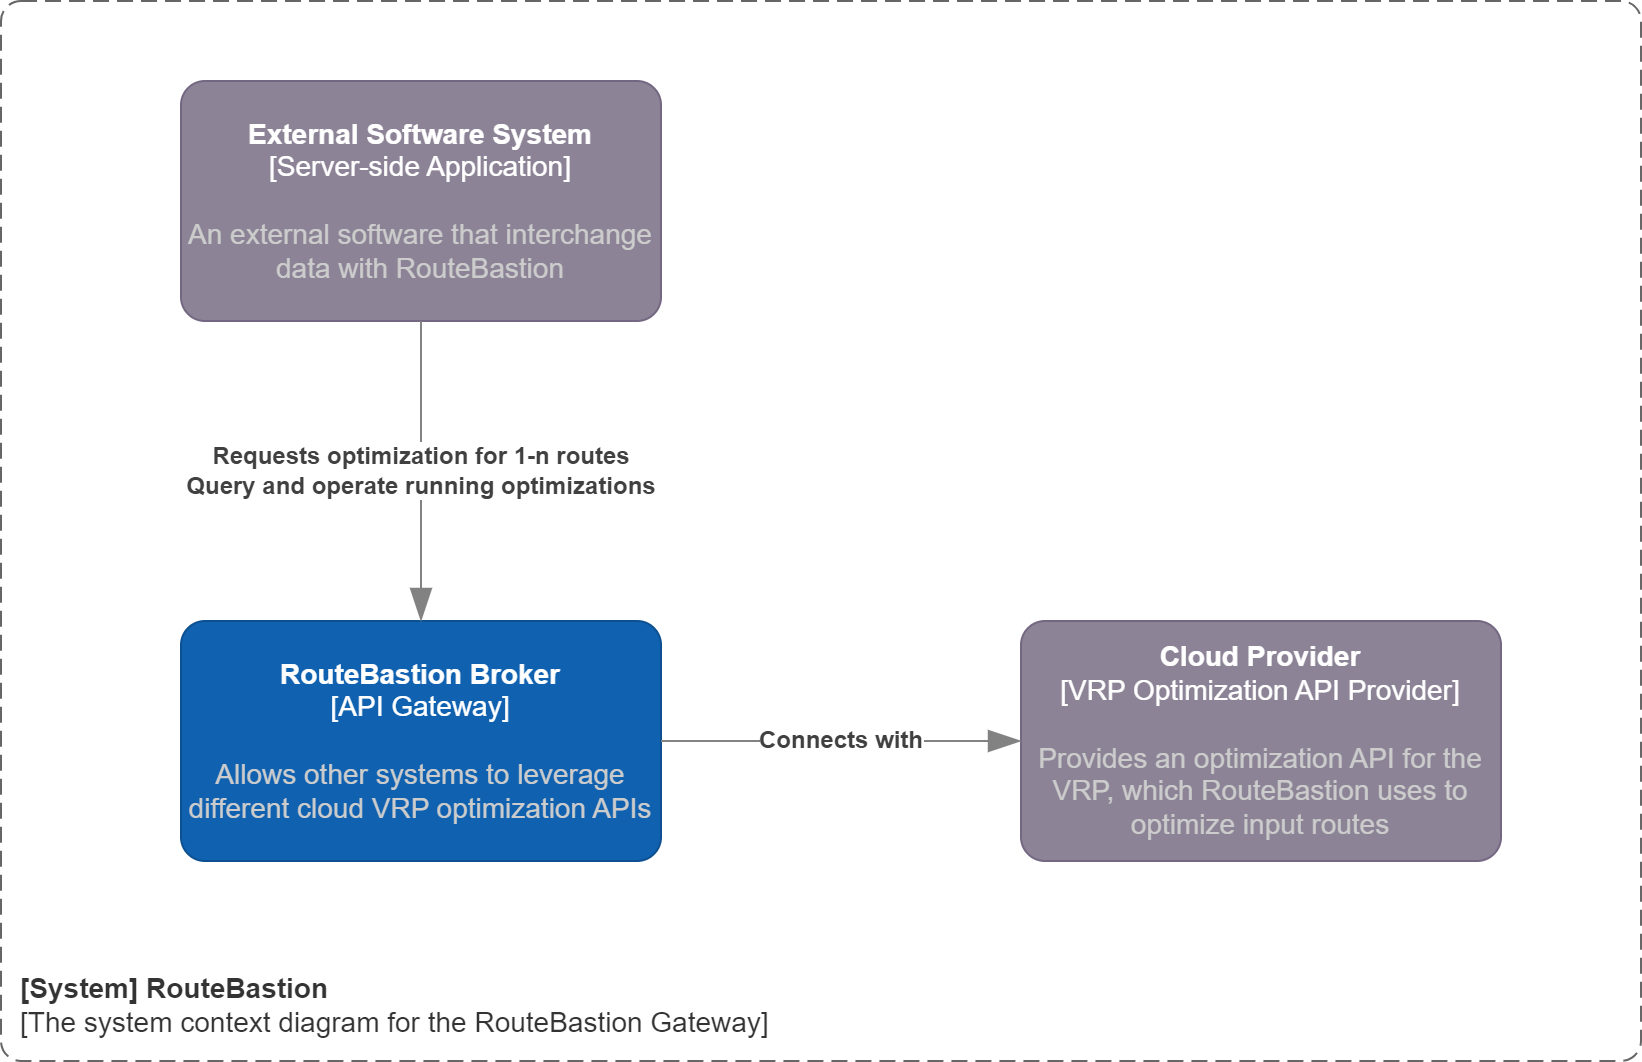
\includegraphics[width=\columnwidth]{figures/c4_diagrams/System_Bigger.png}
  \caption{System Diagram.}
  \label{fig:system}
\end{figure}

% \subsection{Container Architecture}

At the heart of this architecture is the RouteBastion Broker, which serves as the API gateway and manages the selection and routing of optimization requests to the cloud providers. The dynamic cloud provider selection algorithm poses unique challenges, as it must balance performance, cost, and other metrics without introducing significant overhead.

The container diagram, shown in Figure~\ref{fig:container}, delves deeper into the internal components of the RouteBastion Broker system, highlighting the service itself and databases that power the platform. The key components of the architecture include:

\begin{figure}
  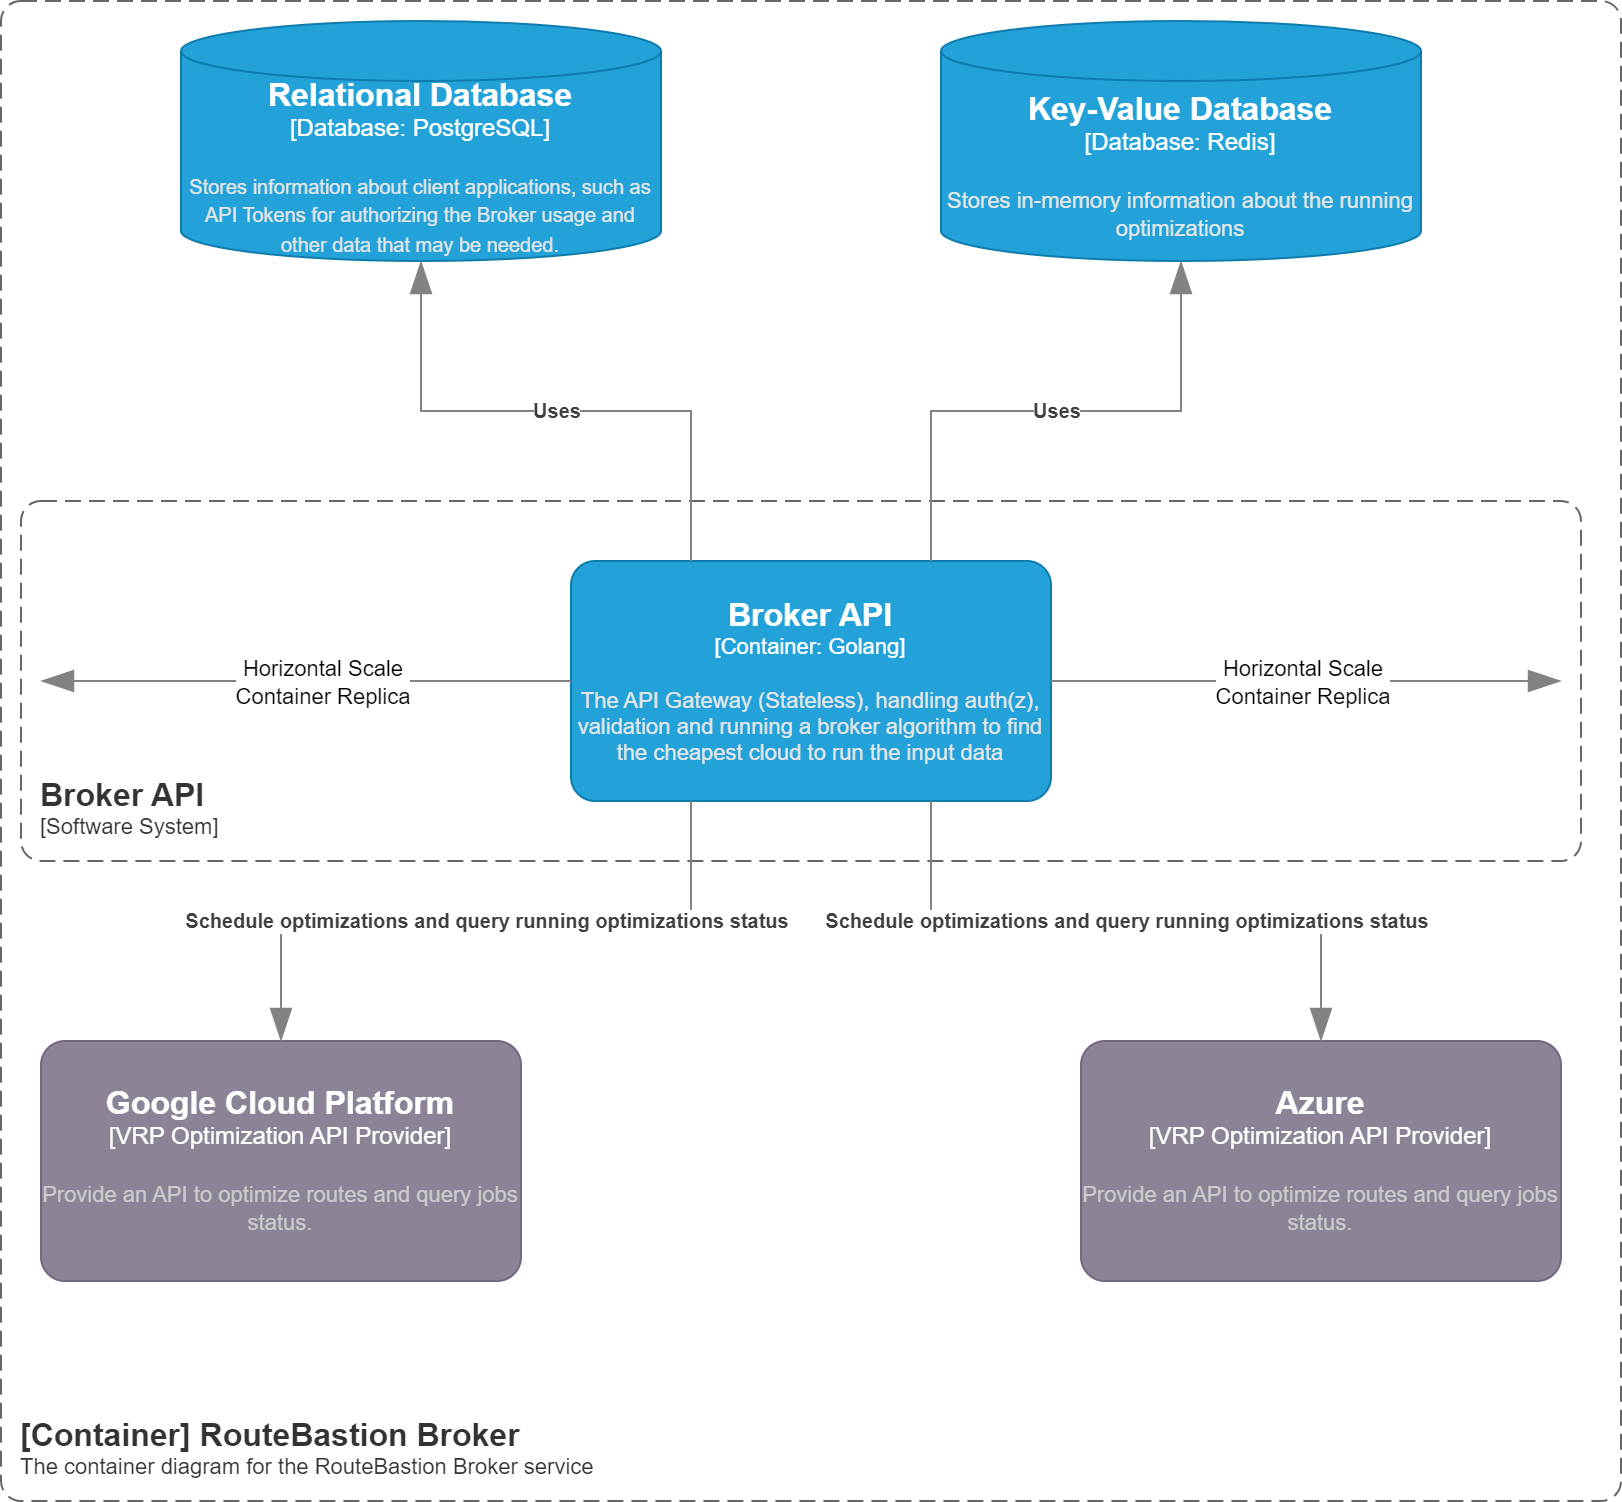
\includegraphics[width=\columnwidth]{figures/c4_diagrams/Container.png}
  \caption{Container Diagram\label{fig:container}}
\end{figure}

\begin{itemize}
  \item \textbf{Broker API}: The Broker API is the main container, which acts as a stateless API gateway, handling authentication/authorization, request validation and running a broker algorithm that dynamically selects a cloud provider. The Broker API is horizontally scalable, meaning that additional replicas can be deployed to handle increased loads, ensuring the system can process high volumes of route optimization requests simultaneously.

  \item \textbf{Relational Database}: This component (e.g., PostgreSQL)  stores persistent data, such as information about client applications (e.g., API tokens for authorization), usage statistics, and other metadata required for managing the system's operations.

  \item \textbf{Key-Value Database}: This component (e.g., Redis) is used to store in-memory data about running optimizations. It allows the system to quickly access real-time information, such as the current status of optimizations, which is essential for monitoring and querying the ongoing optimization processes.

  \item \textbf{Cloud Providers}: These are external services such as Google Cloud and Azure, which provide the actual optimization algorithms and computational power to solve the VRP. The Broker API schedules optimization jobs with these cloud providers and retrieves job statuses, allowing it to present the results back to the external software systems.
\end{itemize}

In summary, while existing systems provide powerful APIs for solving the VRP, RouteBastion differentiates itself by serving as a broker with intelligent, dynamic selection capabilities and a scalable, efficient architecture that optimizes for both performance and flexibility. This introduces new technical challenges, such as state synchronization and decision-making at scale.

\section{Evaluation}
\label{sec:evaluation}


\subsection{Methodology}

% We use the Architecture Tradeoff Analysis Method (ATAM)~\cite{atam} to evaluate the effectiveness and quality of RouteBastion's architecture. ATAM is a structured evaluation technique used to assess the quality attributes of a software architecture by analyzing its trade-offs. It helps stakeholders (such as architects, developers, project managers, clients and virtually any person interested on the software development cycle) identify and prioritize architectural decisions, their effects on the system, and how well the architecture meets various quality attributes such as performance, scalability, modifiability, security, and usability.

% ATAM involves several key steps to systematically evaluate a software architecture. First, the process begins by establishing the context of the architecture, where the business goals, quality attributes (like performance, security, or scalability), and architectural drivers are identified. Next, key stakeholders from different domains (such as developers, architects, and business representatives) are engaged to express their concerns and define quality attribute scenarios, which describe critical use cases or performance goals the system must meet. The architecture is then described in detail, allowing the evaluation team to understand the design decisions made. Following this, architectural scenarios are used to analyze how well the system meets these quality attributes and where potential trade-offs occur between them. The final stages involve identifying sensitivity points (areas where small changes could have a significant impact) and trade-offs (compromises between different quality attributes), as well as prioritizing risks and deciding where further investigation or refinement is needed.

% The Architecture Tradeoff Analysis Method (ATAM) is a structured evaluation technique used to assess the quality attributes of a software architecture. It helps stakeholders like architects, developers, project managers, and clients identify and prioritize architectural decisions, their effects on the system, and how well the architecture meets various quality attributes such as performance, scalability, modifiability, security, and usability. The process begins by establishing the context of the architecture, involving stakeholders from different domains to express concerns and define quality attribute scenarios. The architecture is then described in detail, and potential trade-offs are identified. The final stages involve identifying sensitivity points, trade-offs, prioritizing risks, and deciding where further investigation or refinement is needed. This structured analysis ensures the architecture aligns with business goals while considering the balance between competing system qualities.

We use the Architecture Tradeoff Analysis Method (ATAM)~\cite{atam}, which is a structured evaluation technique used to assess the quality attributes of a software architecture. It helps stakeholders identify and prioritize architectural decisions, their effects on the system, and how well the architecture meets various quality attributes like performance, scalability, modifiability, security, and usability. The process begins with establishing the context of the architecture, engaging stakeholders, and defining quality attribute scenarios. The final stages involve identifying sensitivity points, trade-offs, risks, and prioritizing risks for further investigation or refinement.

\subsection{Architecture Analysis}

\subsubsection{Business Goals and Key Quality Attributes}
\label{subsubsec:bg_kqa}

RouteBastion aims to provide a reliable option to enterprises for selecting the best Cloud Provider for solving Vehicle Routing Problem considering their needs and restrictions. Because of that, the main business goals of our solution are as follows.


% In the ATAM (Architecture Tradeoff Analysis Method), Business Goals represent the overarching objectives of the system from a business or strategic perspective, such as profitability, market growth, or operational efficiency. These goals provide direction and context for why the system is being developed.

% On the other hand, Key Quality Attributes (KQAs) refer to specific, measurable characteristics of the system's architecture that ensure it meets the business goals. These include attributes like performance, security, scalability, and maintainability, which directly influence how the system satisfies its business objectives.

\begin{itemize}
    \item \textbf{Cost-effectiveness}: Selecting the most affordable API for route optimization from multiple cloud providers.
    % \item \textbf{Scalability}: The ability to handle multiple route optimization requests in parallel.
    
    % \item \textbf{Performance}: Ensuring low-latency responses for route optimizations.
   
    \item \textbf{SLA Confidence}: Enhance customer assurance by consistently meeting or exceeding SLA commitments, thereby reinforcing our reputation for reliability and responsiveness in service delivery.
     \item \textbf{Maintainability}: Easy updates and expansions as new cloud providers or APIs become available.
\end{itemize}

We define the following key quality attributes to effectively measure if our systems matches the above goals.

\begin{itemize}
     \item \textbf{Latency}: Measure the overhead on the elapsed time (i.e., delay) from request to response.
    \item \textbf{Scalability and Elasticity}: Measures if the system accommodates fluctuating demand for route optimizations.
    % \item {Performance: To deliver rapid responses from cloud providers and minimize latency.}
    % \item {Modifiability: To easily adapt to changes such as new APIs or business logic.}
    % \item \textbf{Confidentiality}: Measures To ensure client data, including API tokens and route information, are handled securely.
    \item \textbf{Availability}: Measures whether a system is operational and accessible when required.
     \item \textbf{Reliability}: Measures whether a system consistently performs correctly without failure over time
    
\end{itemize}

\subsubsection{Architectural Scenarios}
\label{subsubsec:architectural_scenarios}

Some potential scenarios that stress different quality attributes include:
\begin{itemize}
    \item \textbf{Scenario 1 - API selection based on cost-effectiveness}: The broker must choose the cheapest available API without degrading performance.

    \item \textbf{Scenario 2 - Scalability under high load}:  The RouteBastion Broker receives a large number of route optimization requests concurrently.
    
    \item \textbf{Scenario 3 - Cloud provider failure}: One of the cloud providers is unavailable, and the system must switch to another provider without significant delays.
    \item \textbf{Scenario 4 - Adding a new API provider}: Integrating a new cloud provider into RouteBastion without significant downtime or code changes.
\end{itemize}

\subsubsection{Key Architectural Components and Trade-offs}

Based on section \ref{sec:routebastion} diagrams, we present how our architecture aligns with the quality attributes proposed in section \ref{subsubsec:bg_kqa}, by outlining how each part of it fulfills a key quality attribute.

\paragraph{Broker API} 
% The Broker API is stateless, horizontally scalable, and able to handle multiple requests in parallel. By using Go \cite{gopl}, a language known for its performance and efficient concurrency model (goroutines), this design supports the key quality attributes (KQA) of scalability and elasticity, and availability, by making the architecture easy to scale by adding more instances of the Broker API container. Since Go provides low-latency processing, ideal for minimizing response times in route optimization, it also supports the attribute of latency. The trade-off is that, even though Go provides speed and concurrency, Go’s concurrency model must be carefully managed to avoid potential race conditions under high loads.

The Broker API, using Go \cite{gopl} for its performance and concurrency model, is stateless, horizontally scalable, and capable of handling multiple parallel requests. This design supports key quality attributes (KQA's) of scalability, elasticity, and availability, but requires careful management to avoid race conditions under high loads.

\paragraph{Databases}
% \red{A relational database (PostgreSQL) for persistent storage and a key-value database (Redis) for caching and handling in-memory operations for running optimizations:}

% \red{Performance and Scalability: Redis allows fast lookups and temporary storage of running optimization processes, reducing the load on the PostgreSQL database.}
% \red{Consistency: PostgreSQL offers strong consistency guarantees, which is important for ensuring API tokens and other business-critical data are stored reliably.}
% \red{Trade-off: The separation of data responsibilities between PostgreSQL and Redis introduces complexity, as developers must manage consistency between temporary states in Redis and persistent states in PostgreSQL. Scaling the databases could also become a bottleneck if not carefully managed.}

% The architecture of RouteBastion utilizes a relational database (PostgreSQL) for persistent storage and a key-value database (Redis) for caching and in-memory operations related to running optimizations. This combination supports the KQA's of latency, scalability and availability, as Redis enables fast lookups and temporary storage for ongoing processes, effectively reducing the load on PostgreSQL. Meanwhile, PostgreSQL supports reliability, offering strong guarantees for reliable storage of critical data, such as API tokens and other business-sensitive information. However, this separation of responsibilities introduces a trade-off in terms of complexity, as developers must carefully manage the consistency between the temporary states held in Redis and the persistent data stored in PostgreSQL. Additionally, scaling both databases to handle increased workloads could become a bottleneck if not addressed properly.

RouteBastion's architecture uses PostgreSQL for persistent storage and Redis for caching. This combination supports KQA's latency, scalability, and availability. While Redis reduces load on PostgreSQL, this separation introduces complexity and requires careful management of consistency and scaling for increased workloads.

\paragraph{gRPC and REST}
Using gRPC \cite{grpc} for service-to-service communication between the Broker API, cloud providers and client services supports the KQA of latency. The gRPC's compact binary format (Protocol Buffers) is highly efficient, minimizing overhead compared to REST (which typically uses JSON), providing a greater throughput/sec based on the study of Fakri and Fatih (2024)~\cite{apiGateways}. The trade-offs include the gRPC complexity added to the system and that REST may not be as performant as gRPC during high workloads because of the serialization/deserialization of the JSON payload.

\paragraph{Cloud Provider Integration}
% The architecture is built around the idea of interacting with multiple cloud providers, each providing APIs for route optimization. This idea provides availability and reliability, since the usage of multiple providers provide multiple points of failure for the application, avoiding a full-system shutdown if a single API is unavailable. However, the need to continuously evaluate and switch between different providers introduces potential latency and complexity in decision-making logic. Furthermore, each provider’s API may have different behaviors, requiring extra handling to ensure consistent results across providers.

The architecture uses multiple cloud providers for route optimization, ensuring availability and reliability. However, this approach introduces latency and complexity in decision-making and may require extra handling to ensure consistent results across providers.

\subsection{Discussion}\label{sec:architectural_highlights}

% The goal of optimizing for the cheapest API may sometimes come at the expense of performance. While the system selects the least costly option, switching between APIs could add delays, and lower-cost APIs may have slower response times. The system is horizontally scalable (due to the stateless nature of the Broker API and the use of Redis for caching), ensuring consistency between temporary and persistent states increases the system's complexity. Proper coordination is necessary to avoid issues with data consistency and race conditions. The architecture is flexible enough to add new cloud providers and APIs.

Optimizing for the cheapest API can sometimes compromise performance, as switching between options can cause delays and slower response times. The system is horizontally scalable, but maintaining consistency between temporary and persistent states increases complexity. Proper coordination is necessary to avoid data consistency issues and race conditions. The architecture is flexible enough to accommodate new cloud providers and APIs.

\subsubsection{Sensitivity Points and Risks}

\begin{itemize}
    \item \textbf{Database Bottlenecks}: While Redis helps offload some traffic from PostgreSQL, both databases must be carefully scaled to handle concurrent access under heavy loads.
    \item \textbf{API Decision Logic}: The decision-making logic in the Broker API for selecting the cheapest cloud provider is a critical point of sensitivity. Poor optimization in this algorithm could lead to performance degradation and bias towards a single Cloud Provider. 
    \item \textbf{gRPC Complexity}: While gRPC enhances internal communication, its binary format and the requirement for precise interface definitions (Protobufs) may add development and debugging complexity, particularly for developers more familiar with REST. 
\end{itemize}

\section{Conclusion and Future Work}
\label{sec:conclusion}

% In this paper, we presented the architecture of RouteBastion, which is designed to provide an efficient and scalable solution for optimizing vehicle routing through the integration of various cloud-based APIs. By leveraging the Go programming language for high-performance service execution, REST and gRPC for flexible external/internal communication, RouteBastion ensures that users can seamlessly choose and interact with the most cost-effective and capable cloud provider for their routing needs. Additionally, the potential use of gRPC for internal communication further enhances system performance, allowing the platform to handle large-scale route optimization tasks with minimal latency. This thoughtful combination of technologies positions RouteBastion as a robust and future-proof SaaS offering in the vehicle routing domain.

In this paper, we presented the architecture of RouteBastion, which is designed to provide an efficient and scalable solution through the integration of various cloud-based APIs. The thoughtful combination of technologies positions RouteBastion as a robust and future-proof SaaS offering in the vehicle routing domain.

Future work will concentrate on the Decision-Making Algorithm, the concrete implementation of RouteBastion as a whole, and the improvement of the presented architecture in order to further optimize performance and processes.



\end{document}
